\documentclass[tikz,border=3pt]{standalone}
\usepackage[T1]{fontenc}
\usepackage{lmodern,pgfplots}
\usepgfplotslibrary{groupplots}
\pgfplotsset{compat=1.18}
\begin{document}
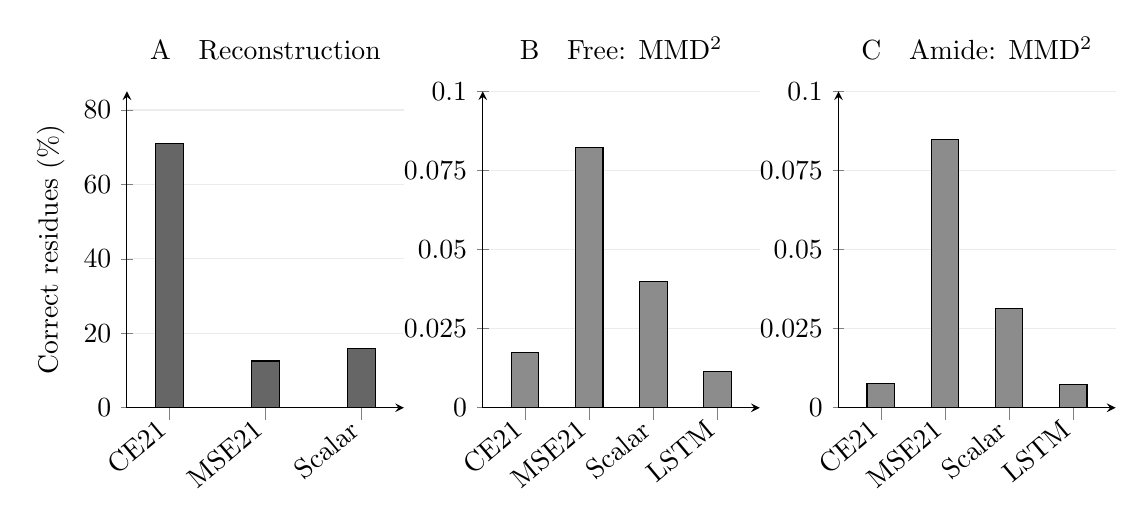
\begin{tikzpicture}
\begin{groupplot}[group style={group size=3 by 1,horizontal sep=1.0cm},width=5.1cm,height=5.6cm,
 tick label style={font=\fontsize{10}{11}\selectfont},label style={font=\fontsize{10}{11}\selectfont},
 title style={font=\fontsize{10}{12}\selectfont,yshift=2pt},
 ymin=0,axis lines=left,xtick=data,xticklabel style={rotate=40,anchor=east},
 enlarge x limits=.22,ymajorgrids=true,grid style={gray!15},
 ybar,/pgf/bar width=10pt,point meta=y]
\nextgroupplot[title={A\quad Reconstruction},ylabel={Correct residues (\%)},ymax=85,
 symbolic x coords={CE21,MSE21,Scalar},ytick={0,20,40,60,80}]
\addplot[fill=black!60,draw=black] coordinates {(CE21,70.8987161198) (MSE21,12.5534950071) (Scalar,15.8345221113)};
\nextgroupplot[title={B\quad Free: MMD$^2$},ymax=.10,
 symbolic x coords={CE21,MSE21,Scalar,LSTM},scaled y ticks=false,ytick={0,.025,.05,.075,.1},
 yticklabel style={/pgf/number format/fixed,/pgf/number format/precision=3}]
\addplot[fill=black!45,draw=black] coordinates {(CE21,.017328) (MSE21,.082335) (Scalar,.039882) (LSTM,.011567)};
\nextgroupplot[title={C\quad Amide: MMD$^2$},ymax=.10,
 symbolic x coords={CE21,MSE21,Scalar,LSTM},scaled y ticks=false,ytick={0,.025,.05,.075,.1},
 yticklabel style={/pgf/number format/fixed,/pgf/number format/precision=3}]
\addplot[fill=black!45,draw=black] coordinates {(CE21,.007710) (MSE21,.084847) (Scalar,.031325) (LSTM,.007362)};
\end{groupplot}
\end{tikzpicture}
\end{document}
